% TODO:
% 1) рассказать ~5 слайдов -- аспекты ``как закодить''













%%%%%%%%%%%%%%%%%%%%%%%%%%%%%%%%%%%%%%%%%
% Beamer Presentation
% LaTeX Template
% Version 1.0 (10/11/12)
%
% This template has been downloaded from:
% http://www.LaTeXTemplates.com
%
% License:
% CC BY-NC-SA 3.0 (http://creativecommons.org/licenses/by-nc-sa/3.0/)
%
%%%%%%%%%%%%%%%%%%%%%%%%%%%%%%%%%%%%%%%%%

%----------------------------------------------------------------------------------------
%	PACKAGES AND THEMES
%----------------------------------------------------------------------------------------

\documentclass{beamer}

\mode<presentation> {

% The Beamer class comes with a number of default slide themes
% which change the colors and layouts of slides. Below this is a list
% of all the themes, uncomment each in turn to see what they look like.

%\usetheme{default}
%\usetheme{AnnArbor}
%\usetheme{Antibes}
%\usetheme{Bergen}
%\usetheme{Berkeley}
%\usetheme{Berlin}
%\usetheme{Boadilla}
%\usetheme{CambridgeUS}
%\usetheme{Copenhagen}
%\usetheme{Darmstadt}
%\usetheme{Dresden}
%\usetheme{Frankfurt}
%\usetheme{Goettingen}
%\usetheme{Hannover}
%\usetheme{Ilmenau}
%\usetheme{JuanLesPins}
%\usetheme{Luebeck}
\usetheme{Madrid}
%\usetheme{Malmoe}
%\usetheme{Marburg}
%\usetheme{Montpellier}
%\usetheme{PaloAlto}
%\usetheme{Pittsburgh}
%\usetheme{Rochester}
%\usetheme{Singapore}
%\usetheme{Szeged}
%\usetheme{Warsaw}

% As well as themes, the Beamer class has a number of color themes
% for any slide theme. Uncomment each of these in turn to see how it
% changes the colors of your current slide theme.

%\usecolortheme{albatross}
%\usecolortheme{beaver}
%\usecolortheme{beetle}
%\usecolortheme{crane}
%\usecolortheme{dolphin}
%\usecolortheme{dove}
%\usecolortheme{fly}
%\usecolortheme{lily}
%\usecolortheme{orchid}
%\usecolortheme{rose}
%\usecolortheme{seagull}
%\usecolortheme{seahorse}
%\usecolortheme{whale}
%\usecolortheme{wolverine}

%\setbeamertemplate{footline} % To remove the footer line in all slides uncomment this line
%\setbeamertemplate{footline}[page number] % To replace the footer line in all slides with a simple slide count uncomment this line

%\setbeamertemplate{navigation symbols}{} % To remove the navigation symbols from the bottom of all slides uncomment this line
}

\usepackage[utf8]{inputenc}
\usepackage[russian]{babel}
\usepackage{cmap}


\usepackage{verbatim}
\usepackage{fancybox}
\usepackage{ulem}
\usepackage{tikz}
\usetikzlibrary{positioning}
\usepackage{scalefnt}
\usetikzlibrary{arrows,shapes,positioning,shadows,trees,calc,backgrounds,fit,positioning}

\usepackage{graphicx} % Allows including images
\usepackage{booktabs} % Allows the use of \toprule, \midrule and \bottomrule in tables
\usepackage{textcomp}
\usepackage{listings}
\usepackage{color}
\usepackage{xcolor}
\usepackage{changepage}

\makeatletter
\newenvironment{noheadline}{
    \setbeamertemplate{headline}{}
    \addtobeamertemplate{frametitle}{\vspace*{-1.6\baselineskip}}{}
}{}
\makeatother

\definecolor{mygreen}{rgb}{0,0.6,0}
\definecolor{mygray}{rgb}{0.5,0.5,0.5}
\definecolor{mymauve}{rgb}{0.58,0,0.82}

\lstset{ %
  backgroundcolor=\color{white},   % choose the background color; you must add \usepackage{color} or \usepackage{xcolor}
  basicstyle=\footnotesize,        % the size of the fonts that are used for the code
  breakatwhitespace=false,         % sets if automatic breaks should only happen at whitespace
  breaklines=true,                 % sets automatic line breaking
  captionpos=b,                    % sets the caption-position to bottom
  commentstyle=\color{mygreen},    % comment style
  deletekeywords={...},            % if you want to delete keywords from the given language
  escapeinside={\%*}{*)},          % if you want to add LaTeX within your code
  extendedchars=true,              % lets you use non-ASCII characters; for 8-bits encodings only, does not work with UTF-8
  frame=single,                    % adds a frame around the code
  keepspaces=true,                 % keeps spaces in text, useful for keeping indentation of code (possibly needs columns=flexible)
  keywordstyle=\color{blue},       % keyword style
  language=Octave,                 % the language of the code
  morekeywords={*,...},            % if you want to add more keywords to the set
  numbers=left,                    % where to put the line-numbers; possible values are (none, left, right)
  numbersep=5pt,                   % how far the line-numbers are from the code
  numberstyle=\tiny\color{mygray}, % the style that is used for the line-numbers
  rulecolor=\color{black},         % if not set, the frame-color may be changed on line-breaks within not-black text (e.g. comments (green here))
  showspaces=false,                % show spaces everywhere adding particular underscores; it overrides 'showstringspaces'
  showstringspaces=false,          % underline spaces within strings only
  showtabs=true,                  % show tabs within strings adding particular underscores
  stepnumber=1,                    % the step between two line-numbers. If it's 1, each line will be numbered
  stringstyle=\color{mymauve},     % string literal style
  tabsize=4,                       % sets default tabsize to 2 spaces
  %title=\lstname                   % show the filename of files included with \lstinputlisting; also try caption instead of title
}

\graphicspath{{./figures/}}

%----------------------------------------------------------------------------------------
%	TITLE PAGE
%----------------------------------------------------------------------------------------

\title[Обработка и исполнение запросов: лекция 9]{Обработка и исполнение запросов в СУБД (Лекция 9) \\~\\ XML СУБД\\~\\ v6} % The short title appears at the bottom of every slide, the full title is only on the title page

\author{Георгий Чернышев} % Your name
\institute[ВШЭ] % Your institution as it will appear on the bottom of every slide, may be shorthand to save space
{
Высшая Школа Экономики \\ % Your institution for the title page
\medskip
\textit{chernishev@gmail.com} % Your email address
}
\date{\today} % Date, can be changed to a custom date

\date{18 ноября 2020 г.}

\begin{document}

\begin{frame}
\titlepage % Print the title page as the first slide
\end{frame}

\begin{comment}
\begin{frame}
\frametitle{Overview} % Table of contents slide, comment this block out to remove it
\tableofcontents % Throughout your presentation, if you choose to use \section{} and \subsection{} commands, these will automatically be printed on this slide as an overview of your presentation
\end{frame}
\end{comment}

\begin{frame}
\frametitle{План лекции}

\begin{itemize}
  \setlength\itemsep{1em}
  \item Модель данных XML;
  \item Языки запросов к XML;
  \item Три подхода к выполнения запросов к XML: 
  \begin{enumerate}
    \item Реляционные XML процессоры;
    \item Нативные XML процессоры;
    \item Смешанная схема.
  \end{enumerate}
  \item Индексирование для XPath;
  \item Выполнение XPath запросов на примере алгоритмов PathStack и TwigStack;
  \item Итог: настоящее XML и будущее древовидных моделей данных.
\end{itemize}
\end{frame}

\begin{frame}
\frametitle{XML I}

\begin{itemize}
  \setlength\itemsep{1em}
  \item XML~--- eXtensible Markup Language;
  \item Бесплатное упрощение ISO Standard General Markup Language (SGML); первая версия вышла в 1998, W3C;
  \item Идеи: 
  \begin{enumerate}
    \item добавим к тексту теги, для возможности придания семантики;
    \item дать возможность пользователю задавать свои теги;
    \item текст должен быть читабельным пользователем;
    \item возможность указания обработки;
  \end{enumerate}
  \item Пришел не один, а с ``обвесом'' других языков и технологий;
  \item Формирует базис многих технологий: ODF, XHTML, OOXML, DocBook.
\end{itemize}
\end{frame}

\begin{frame}
\frametitle{XML II}

Успешные приложения:

\begin{itemize}
  \setlength\itemsep{1em}
  \item Собственно, разметка документов;
  \item Обмен данными в слабо связанных системах:
  \begin{itemize}
    \item DTD или XML Schema задает формат сообщений при общении различных компьютерных систем;
    \item То есть, XML описывает формат, структуру и данные сообщений;
    \item Примеры: SOAP, RSS/Atom.
  \end{itemize}
  \item Моделирование слабо-структурированных данных:
  \begin{itemize}
    \item Суть: менее строгая нежели реляционная, ER и OO модели;
    \item Иерархическая, гибкая, позволяет разреженность в данных;
    \item Позволяет иметь гетерогенную структуру данных;
    \item Позволяет иметь свои свойства для каждого объекта;
    \item Способна к быстрым изменениям.
  \end{itemize}  
\end{itemize}
\end{frame}

% todo: схема

\begin{frame}[fragile]
\frametitle{XML III}

\lstset{language=XML}   

\begin{itemize}
  %\setlength\itemsep{1em}
  \item Элемент (открывающий и закрывающий тег + тело):
  \begin{lstlisting}
  <t1> body </t1>\end{lstlisting}  
  \item Элементы могут быть вложенными:
  \begin{lstlisting}
  <t1> body1 <t2> body2 </t2> </t1>\end{lstlisting}    
  \item Тег может иметь атрибуты:
  \begin{lstlisting}
  <t1 attr1=``value1''> body </t1>\end{lstlisting}    
  \item Элементы могут быть пустыми:
  \begin{lstlisting}  
  <t1/>\end{lstlisting}      
  \item DTD и XML schema ограничивают возможные деревья;
  \item В дереве есть порядок, левосторонний обход в глубину.
\end{itemize}
\end{frame}


\begin{frame}[t]
\frametitle{Пример I}

Пример взят из \url{http://www.w3schools.com/xml/xquery_example.asp}

\begin{tikzpicture}[remember picture,overlay]
    \node[xshift=-9.0cm,yshift=-5cm] at (current page.north east) {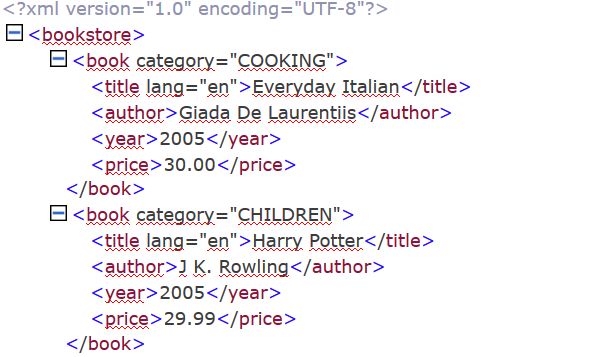
\includegraphics[width=7cm]{xml-code1.png}};
\end{tikzpicture}

\begin{tikzpicture}[remember picture,overlay]
    \node[xshift=-3.0cm,yshift=-6cm] at (current page.north east) {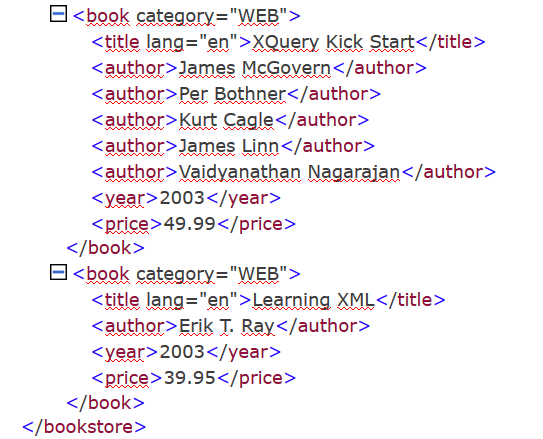
\includegraphics[width=7cm]{xml-code2.png}};
\end{tikzpicture}

%\begin{figure}[htb]
%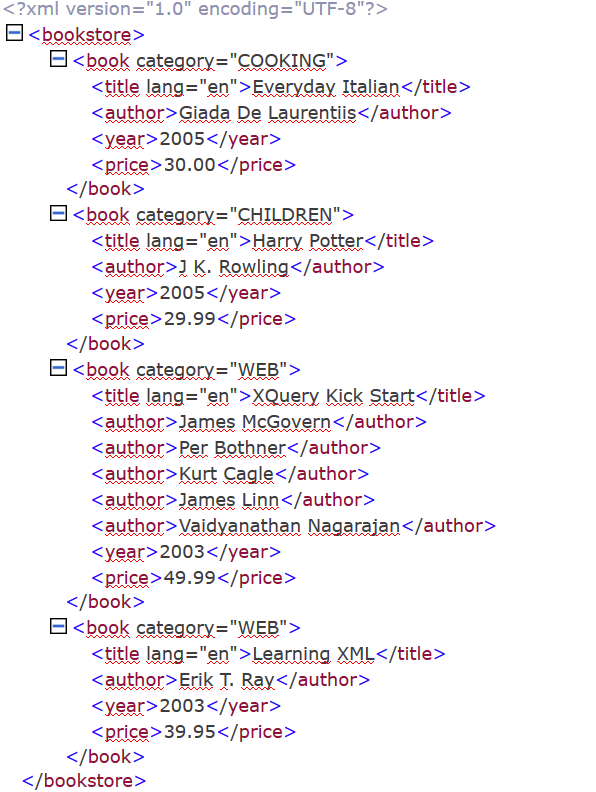
\includegraphics[width=\textwidth,height=0.850\textheight,keepaspectratio]{xml-code.png} 
%\footnote{\tiny{Изображение взято из \cite{Harizopoulos2009}}}
%\end{figure}    
  
\end{frame}

\begin{frame}[t]
\frametitle{Пример II}

\begin{figure}[htb]
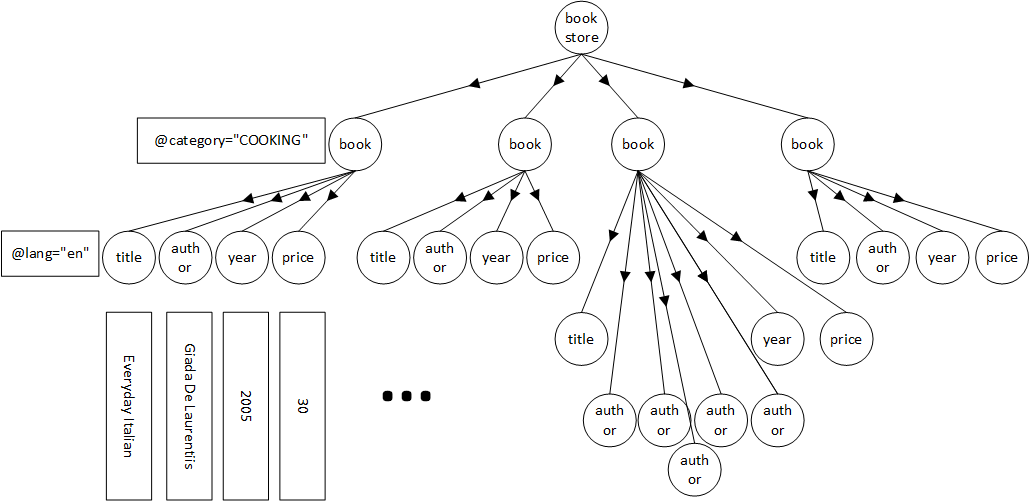
\includegraphics[width=\textwidth,height=0.850\textheight,keepaspectratio]{xml-pic.png} 
\end{figure}    
  
\end{frame}

\begin{frame}
\frametitle{Языки запросов к XML \cite{Hidders2009}}

\begin{itemize}
  \setlength\itemsep{1em}
  \item XPath (XML path language)~--- язык навигационных выражений
  \begin{itemize}
    \item разрабатывался W3C, с 1999 года;
    \item поиск шаблона в графе;
    \item последовательность шагов для выборки узлов.
  \end{itemize}
  \item XQuery (XML query language)~--- декларативный язык для запросов к коллекциям XML документов;
  \begin{itemize}
    \item тоже W3C, 1998;
    \item появился не на пустом месте: Quilt, Lorel, YATL;
    \item подобен SQL, формула FLWOR;
    \item включает в себя XPath.
  \end{itemize}
  
  \item Множество других, нишевых: XUpdate, NEXI, XQuery Full-Text, ...
\end{itemize}
\end{frame}

\begin{frame}[fragile]
\frametitle{XPath}

Последовательность location steps, формируем путь наподобие пути к каталогу в linux:

\lstset{language=XML}
\begin{itemize}
  \setlength\itemsep{1em}
  \item Может быть абсолютным, а может быть относительным;
  Пример: 
  \begin{lstlisting}
  book/title/@lang
  /bookstore/book/title/@lang\end{lstlisting}  
  \item * и @* для всех элементов и атрибутов;
  \item другие: //, .., |
  \item предикаты: 1) сравнение строк 2) существование 3) позиционные
  \begin{lstlisting}
  //title[@lang=``en'']/..
  //book[author=``J K. Rowling'' and price<30]
  //book/author[2]
  //book[/author]
  //book[/author]/price\end{lstlisting}  
  
\end{itemize}
\end{frame}

\begin{frame}[fragile]
\frametitle{XPath: еще примеры}

\lstset{language=XML} 

Запрос 1: doc("books.xml")/bookstore/book/title 

\begin{lstlisting}
<title lang="en">Everyday Italian</title>
<title lang="en">Harry Potter</title>
<title lang="en">XQuery Kick Start</title>
<title lang="en">Learning XML</title> 
\end{lstlisting}


Запрос 2: doc("books.xml")/bookstore/book[price<30] 



\begin{lstlisting}
<book category="CHILDREN">
  <title lang="en">Harry Potter</title>
  <author>J K. Rowling</author>
  <year>2005</year>
  <price>29.99</price>
</book> 
\end{lstlisting}


\end{frame}


\begin{frame}[fragile]
\frametitle{XQuery I}

FLOWR нотация:

\begin{itemize}
  %\setlength\itemsep{1em}
  \item FOR~--- выборка последовательности узлов;
  \item LET~--- привязка последовательности к переменной;
  \item WHERE~--- фильтрация узлов;
  \item ORDER BY~--- сортировка узлов;
  \item RETURN~--- что возвращать (вычисляется один раз для каждого узла).
\end{itemize}

Пример 1:
\lstset{language=XML} 
\begin{lstlisting}
for $x in doc("books.xml")/bookstore/book
where $x/price>30
return $x/title 
\end{lstlisting}
Результат:
\begin{lstlisting}
<title lang="en">XQuery Kick Start</title>
<title lang="en">Learning XML</title> 
\end{lstlisting}

\end{frame}

\begin{frame}[fragile]
\frametitle{XQuery II}

Пример 2:
\lstset{language=XML} 
\begin{lstlisting}
for $x in doc("books.xml")/bookstore/book
where $x/price>30
order by $x/title
return $x/title 
\end{lstlisting}
Результат:
\begin{lstlisting}
<title lang="en">Learning XML</title> 
<title lang="en">XQuery Kick Start</title>
\end{lstlisting}
XPath аналог так не может:
\begin{lstlisting}
doc("books.xml")/bookstore/book[price>30]/title 
\end{lstlisting}


\end{frame}

\begin{frame}[fragile]
\frametitle{XQuery III}

FLOWR нотация:

\begin{itemize}
  %\setlength\itemsep{1em}
  \item В FOR и LET может быть несколько последовательностей;
  \item В RETURN может быть IF или CASE;
  \item В FLOWR узлы можно создавать на лету;
  \item ...
\end{itemize}

Пример 3:
\lstset{language=XML} 
\begin{lstlisting}
for $s in fn:doc(``students.xml'')//student,
     $e in fn:doc(``enrollments.xml'')//enrollment
let $cn := fn:doc(``courses.xml'')//course[@crs-code=$e/@crs-code]/name
where $s/@stud-id = $e/@stud-id
order by $cn
return <enroll> {$s/name, $cn} </enroll>
\end{lstlisting}

%Замечание: XQuery~--- Тьюринг-полный.

\end{frame}

\begin{frame}
\frametitle{XQuery: выполнение \cite{Grust2009}}

Как можно строить XML СУБД:

\begin{enumerate}
 \setlength\itemsep{1em}

  \item Использовать реляционную СУБД: оттранслировать XML в таблицы, оттранслировать запрос в SQL, выполнить, оттранслировать результаты в XML и выдать обратно;
  \item Выполнять нативно. Требуются специальные методы индексирования и выполнение запросов;
  \item Гибридная схема, смесь реляционных подходов и XML технологий.
\end{enumerate}

\end{frame}

\begin{frame}[t]
\frametitle{Примеры систем}

\begin{figure}[htb]
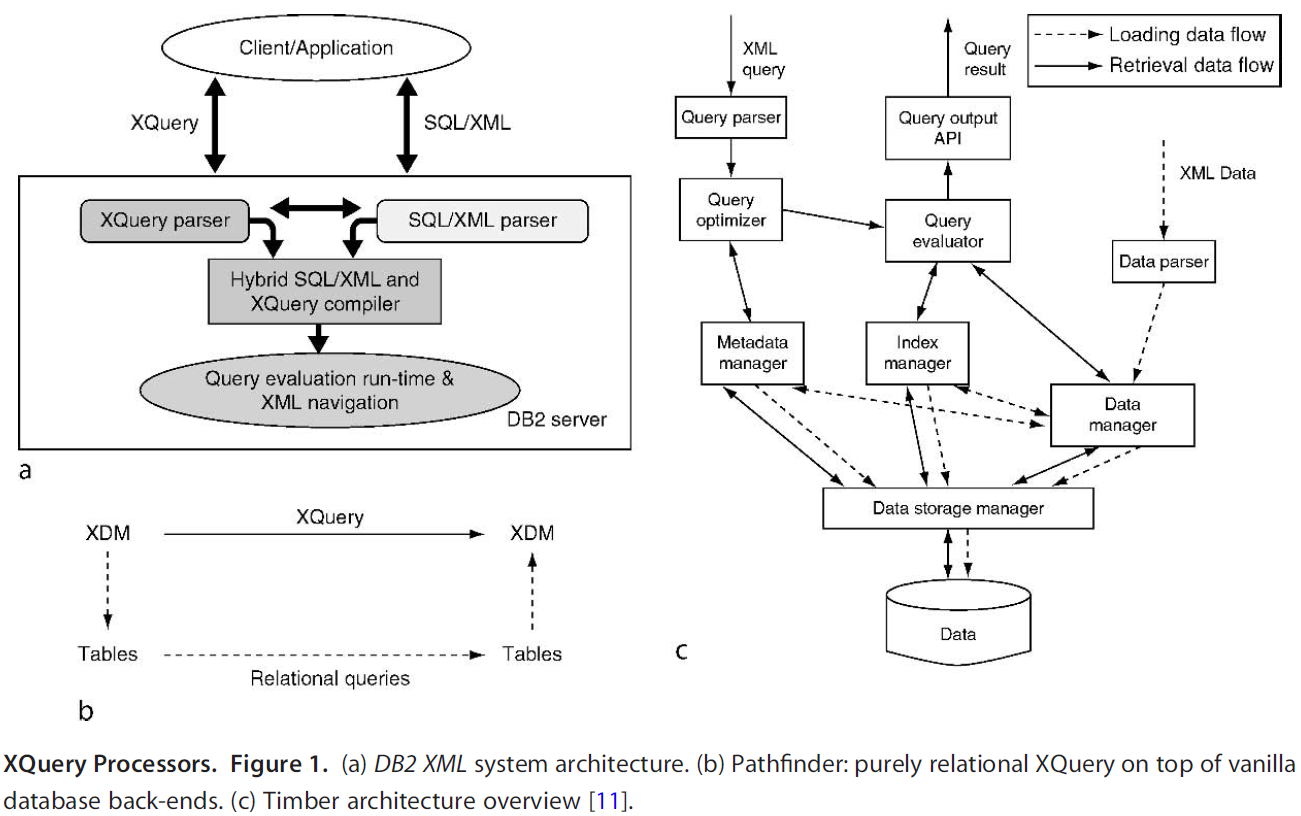
\includegraphics[width=\textwidth,height=0.77\textheight,keepaspectratio]{xml-approaches.png} 
\footnote{\tiny{Изображение взято из \cite{Grust2009}}}
\end{figure}    
  
\end{frame}

\begin{frame}
\frametitle{Реляционные СУБД и XML}
Pathfinder: чисто реляционное выполнение XQuery
\begin{itemize}
  \setlength\itemsep{1em}
  \item Идея: существующие реляционные системы могут эффективно исполнять XQuery;
  \item В основе XQuery лежит понятие секвенции~--- последовательность состоящая из значений и деревьев. Для кодирования секвенций:
  \item Модель XDM (XQuery Data Model)~--- каждый узел это запись в таблице, возможно, с ``хитрой'' системой кодирований (pre/post region\footnote{\url{http://db.in.tum.de/~grust/files/xquery-on-sql-hosts.pdf} материалы школы EDBT}, ORDPATH) \cite{Grust2009};
  \item Вычисление запроса: результаты FOR (для каждой переменной) выкладываем в таблицу, ``разворачивая'' их;
  \item Далее, на эту таблицу надстраиваем операторы специальной алгебры (Flat Relational Algebra).
\end{itemize}
\end{frame}



\begin{frame}[t]
\frametitle{Pathfinder: кодирование последовательностей}

\begin{figure}[htb]
	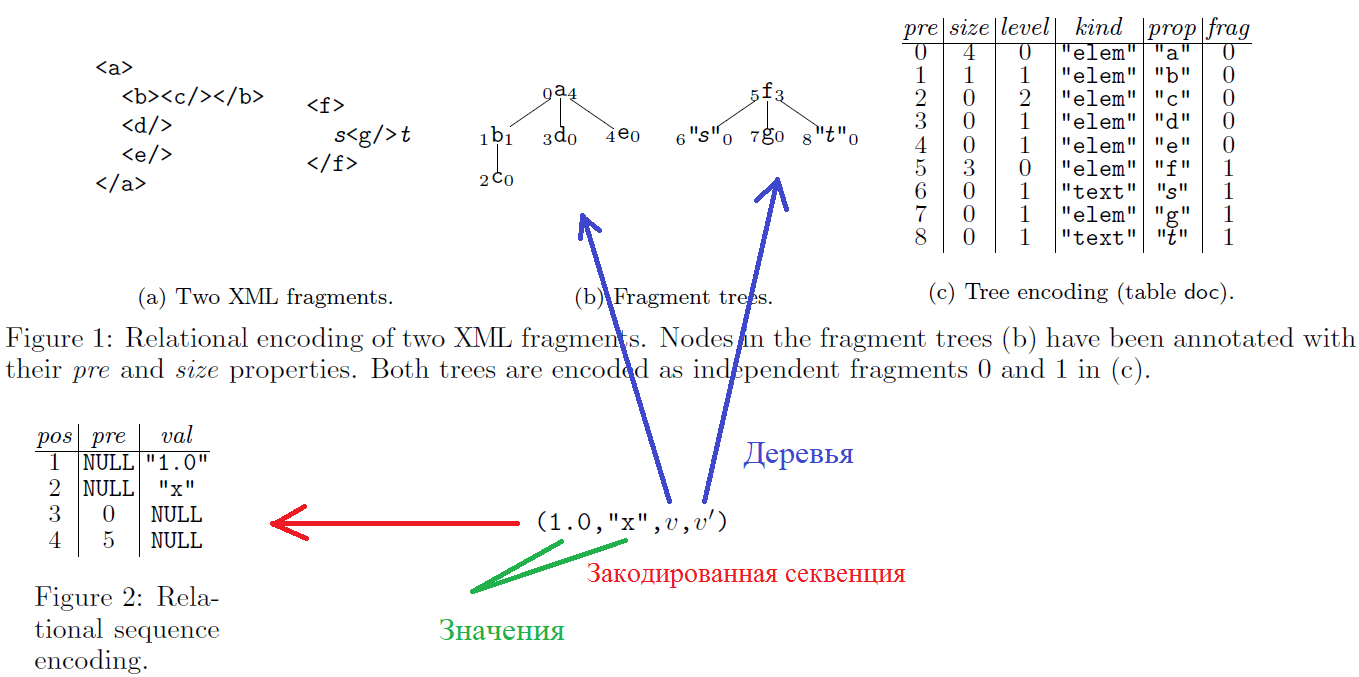
\includegraphics[width=\textwidth,height=0.77\textheight,keepaspectratio]{pathfinder-coding.png} 
	\footnote{\tiny{Изображение взято из~\cite{Grust2004}}}
\end{figure}

\end{frame}

\begin{frame}[t]
\frametitle{Pathfinder (выполнение FLOWR): пример I}

\begin{figure}[htb]
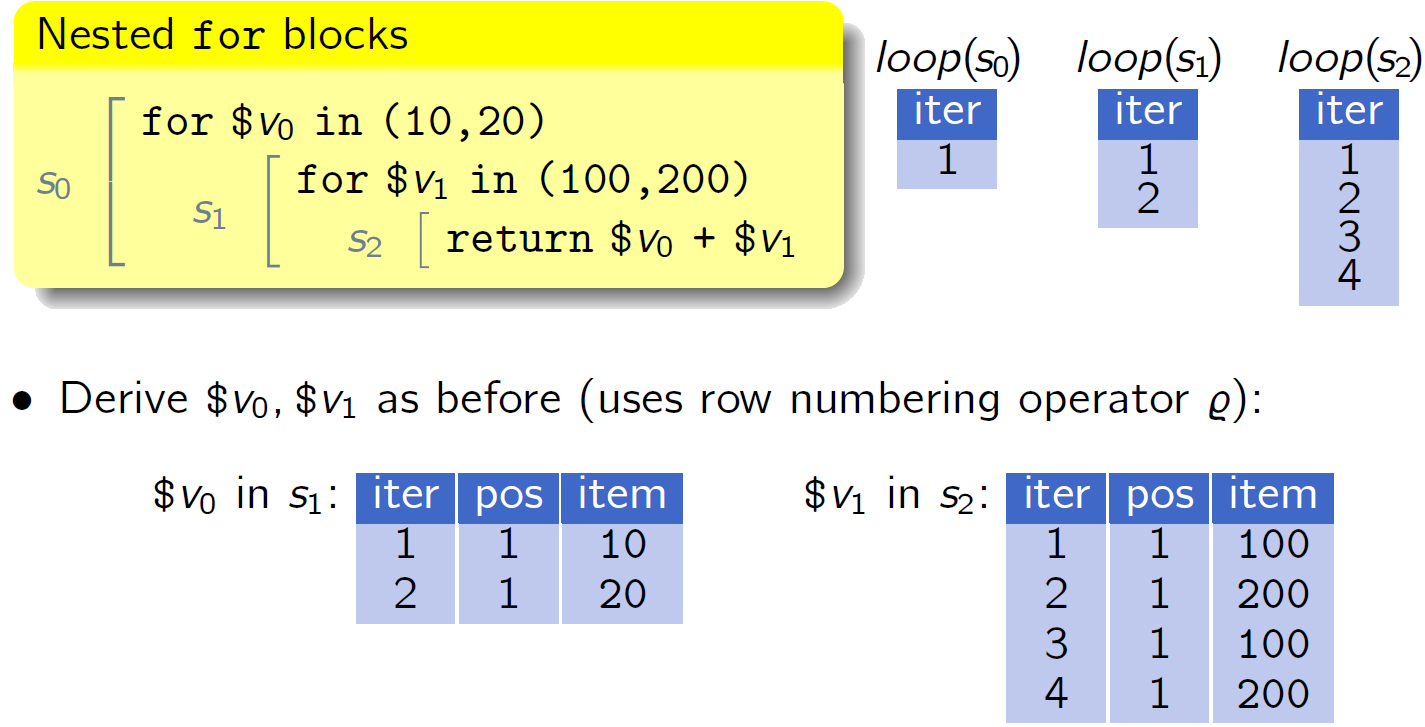
\includegraphics[width=\textwidth,height=0.77\textheight,keepaspectratio]{pathfinder.png} 
\footnote{\tiny{Изображение взято из \url{http://db.in.tum.de/~grust/files/xquery-on-sql-hosts.pdf}}}
\end{figure}
  
\end{frame}

\begin{frame}[t]
\frametitle{Pathfinder (выполнение FLOWR): пример II}

\begin{figure}[htb]
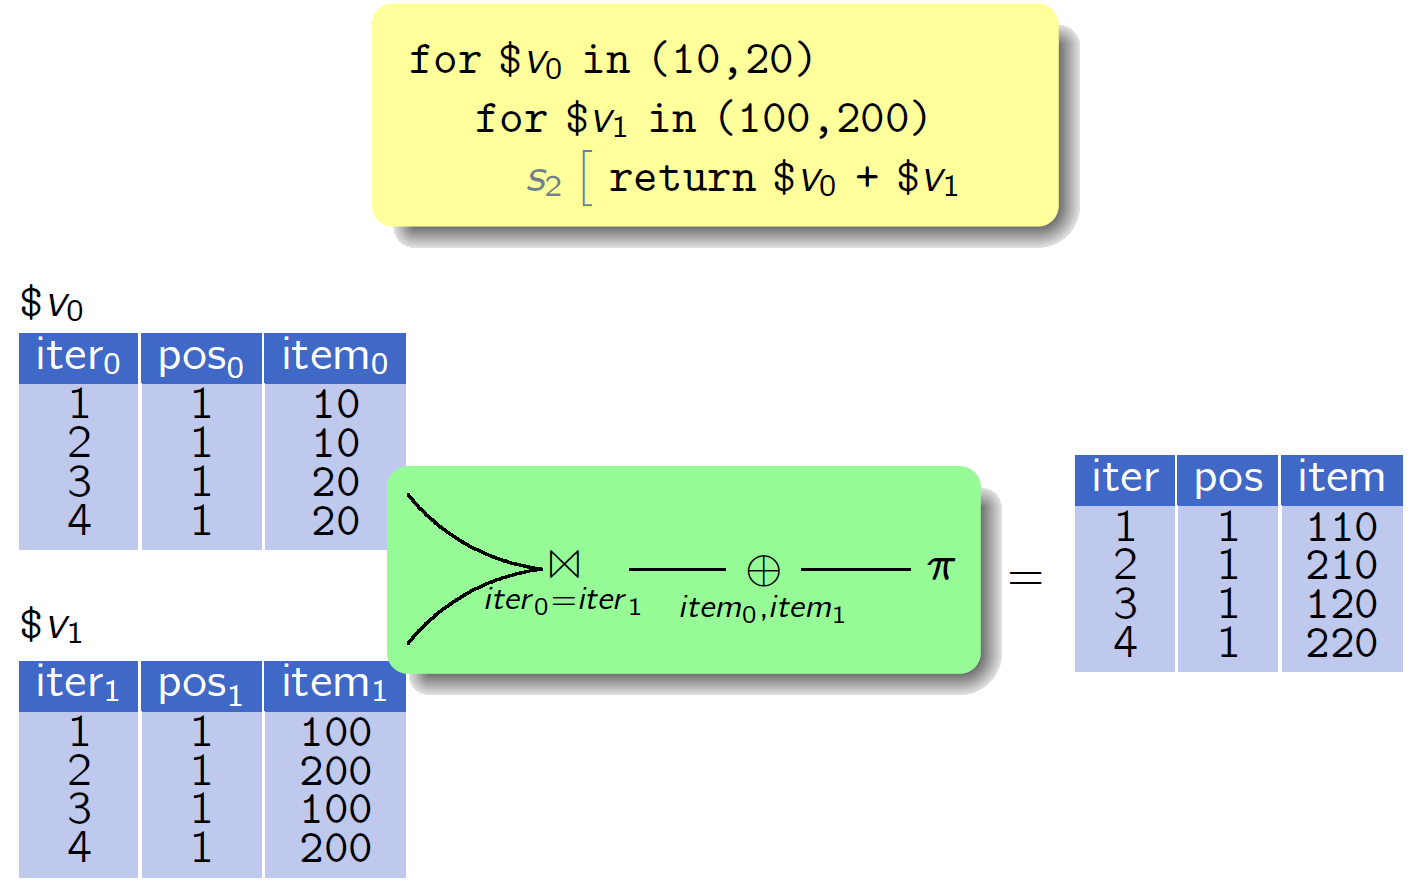
\includegraphics[width=\textwidth,height=0.63\textheight,keepaspectratio]{pathfinder2.png} 
\footnote{\tiny{Изображение взято из \url{http://db.in.tum.de/~grust/files/xquery-on-sql-hosts.pdf}}}
\end{figure}    

Кому непонятно имеет смысл глянуть еще вот сюда: "Pathfinder: XQuery - The Relational Way".
  
\end{frame}

\begin{frame}
\frametitle{DB2 XML: гибрид реляционной и XML СУБД}
Идея: реляционные и XML данные могут успешно дополнять друг с друга, но XML данные потребуют свого хранилища и процессора. Реляционные компоненты остаются и переиспользуются. $\longrightarrow$ Можно использовать оба типа данных вместе (SQL + XQuery или SQL/XML).

\begin{itemize}
  %\setlength\itemsep{0.5em}
  \item Хранит двоичное представление XML дерева, не надо парсить;
  \item Запросы не в SQL, а в свой Query Graph Model (QGM);
  \item Была перезапись запроса и стоимостная оптимизация для XQuery;
  \item Не сильно зависит от схемы, но использует для выбора индексов;
  \item Индексы для XPath выражений: 
  \begin{itemize}
    \item строится для выражения, умеет /, //, [ ];
    \item представлен как два $B^{+}$-дерева~--- path, value index;
    \item path index~--- все различные пути, в path id;
    \item value index~--- содержит path id, значения, и node id~--- для каждого узла, удовлетворяющего индексируемому выражению;     
    \item так как индексы строятся на сложных XPath выражениях, предложили алгоритм проверки вложенности деревьев для выбора индекса;
  \end{itemize}
\end{itemize}
\end{frame}

\begin{frame}
\frametitle{Нативные XML СУБД \cite{Grust2009}}

\begin{itemize}
  \setlength\itemsep{1em}
  \item XML данные хранятся в их естественном виде, нет затрат на конвертацию в SQL и обратно;
  \item Примеры: Timber \cite{Jagadish2002} и Sedna \cite{Taranov2010}
  \item В Timber~--- своя алгебра для работы с XML: access methods, методы перезаписи запроса и стоимостная оптимизация;
  \item При загрузке документа узлу сопоставляется (D, S, E, L): Document, Start Key, End Key, Level (node);
  \item Эта схема позволяет быстро устанавливать отношения между узлами:
  \begin{itemize}
    \item $<d_1, s_1, e_1, l_1>$ предок $<d_2, s_2, e_2, l_2> \iff (s_1 < s_2)\, \& \, (e_1 > e_2)$
  \end{itemize}
  \item Узлы хранятся в порядке Start key.
\end{itemize}
\end{frame}

\begin{frame}
\frametitle{Timber}

\begin{itemize}
  \setlength\itemsep{1em}
  \item Представление XQuery~--- алгебра TLC (Tree Logical Class), оперирует последовательностями упорядоченных, помеченных деревьев;

  \begin{itemize}
	\item операторы: filter, select, project, join, ... , flatten, shadow/illuminate.  	
\end{itemize}

  
  
  \item TIX~--- алгебра-расширение для систем информационного поиска, добавили функции оценки;
  \item Новые физические операторы: материализация узла (по id узла получить поддерево), структурное соединение (вычисление XPath) ~--- набор stack-based алгоритмов;
  \item Оптимизатор: 1) когда материализовывать, 2) последовательность структурных соединений~--- выбор порядка их проведения;
  \item Оптимизатор~--- стоимостной, оценка результата основывается на специализированной гистограмме для XML (positional histogram).
\end{itemize}
\end{frame}

\begin{frame}
	\frametitle{Sedna}
	
	\begin{itemize}
		\setlength\itemsep{1em}
		\item Делал коллектив в ИСПРАН, руководитель~--- С.Д.~Кузнецов (его переводы я отсылал вас читать на citforum).
		\item Активная разработка 2004--2008, 2006/7 -- OpenSource.
		\item Централизованная, дисковая (делали pointer swizzling).
		\item Было:
		\begin{itemize}
			\item 100\% поддержка XQuery,
			\item транзакции,
			\item внедрения (Большая Российская Энциклопедия, для нее вкрутили полнотекстовый поиск).
		\end{itemize}
		\item На мой взгляд это самый большой контрибьшен в исследовательское сообщество по базам данных, за всю историю страны.
		\item Их пытался купить Оракл (!).
	\end{itemize}
\end{frame}


%\begin{frame}
%\frametitle{Recycler II: идея}

%\begin{itemize}
%  \setlength\itemsep{1em}
%  \item ???
%\end{itemize}
%\end{frame}

\begin{frame}
\frametitle{Немного про индексирование XPath}

По \cite{Luna2009}:

\begin{itemize}
  \setlength\itemsep{1em}
  \item Индексирование вершин (схемы нумерации вершин):
  \begin{itemize}
    \item ID~--- в лоб: подобие инвертированного индекса, но это дорого :(
    \item Dewey~--- аналог библиотечной классификации, проверка подстроки (делаем trie), плоха если дерево глубокое;
    \item Интервальная схема~--- тройки из (первая нумерация, вторая нумерация, первая нумерация родителя) при левостороннем обходе;
    \begin{itemize}
      \item проверять вложенность для потомка, для ребенка равенство;
      \item потом на интервалах можно сделать R-tree;
    \end{itemize}    
  \end{itemize}
  \item Индексирование путей: записать путь от одной вершины и до другой.
\end{itemize}
\end{frame}

\begin{frame}
\frametitle{Исходные данные:}
\begin{figure}[htb]
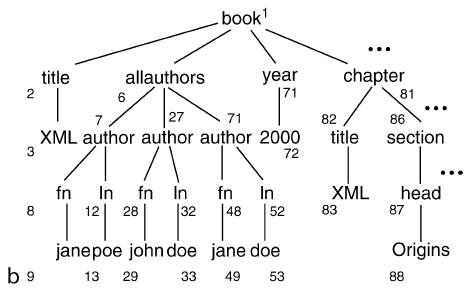
\includegraphics[width=\textwidth,height=0.65\textheight,keepaspectratio]{xml-id.png} 
\footnote{\tiny{Изображение взято из \cite{Luna2009}}}
\end{figure}    
\end{frame}

\begin{frame}
\frametitle{Схема Dewey}
\begin{figure}[htb]
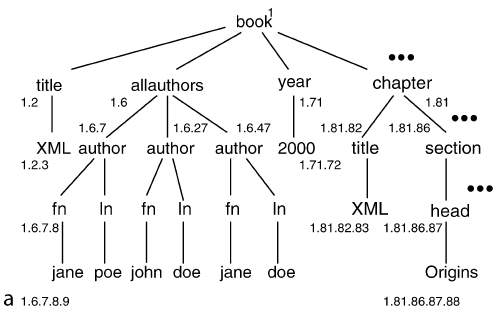
\includegraphics[width=\textwidth,height=0.65\textheight,keepaspectratio]{xml-dewey.png} 
\footnote{\tiny{Изображение взято из \cite{Luna2009}}}
\end{figure}    
\end{frame}

\begin{frame}
\frametitle{Интервальная схема}
\begin{figure}[htb]
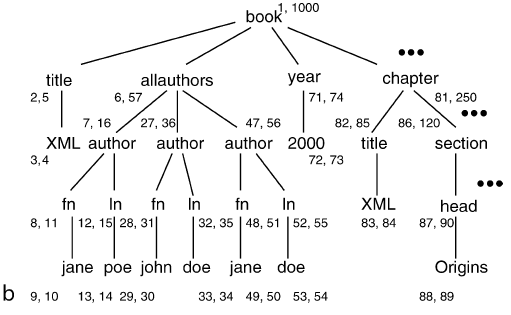
\includegraphics[width=\textwidth,height=0.65\textheight,keepaspectratio]{xml-interval.png} 
\footnote{\tiny{Изображение взято из \cite{Luna2009}}}
\end{figure}    
\end{frame}

\begin{frame}
\frametitle{Индексирование путей}
\begin{figure}[htb]
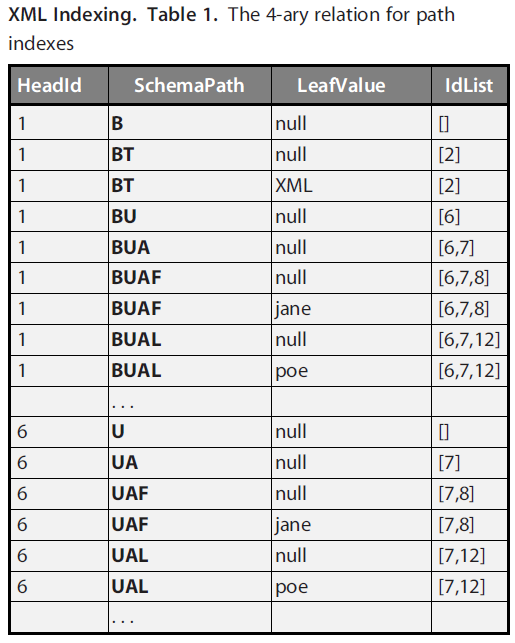
\includegraphics[width=\textwidth,height=0.80\textheight,keepaspectratio]{xml-pathindex.png} 
\footnote{\tiny{Изображение взято из \cite{Luna2009}}}
\end{figure}    
\end{frame}

\begin{frame}
\frametitle{Схема методов для подхода индексирования путей}
\begin{figure}[htb]
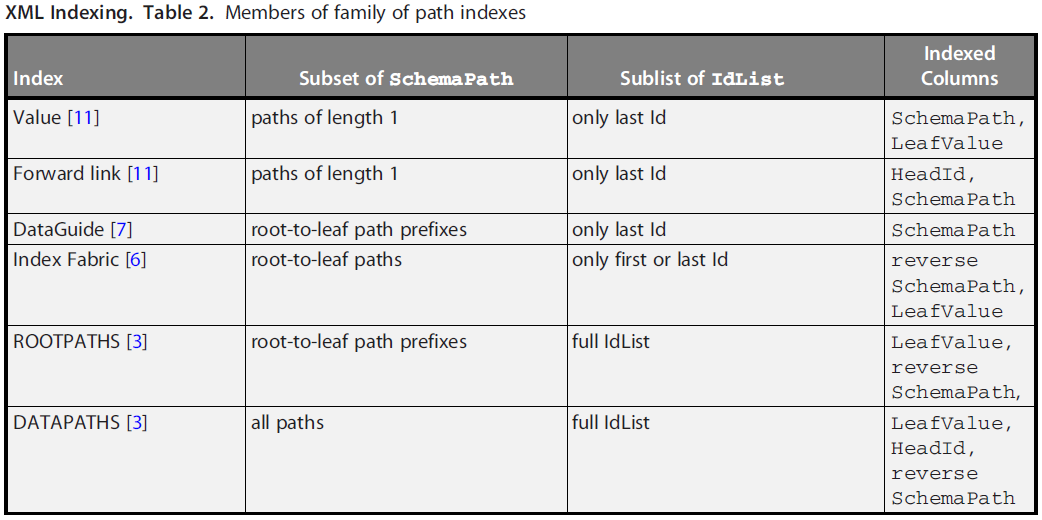
\includegraphics[width=\textwidth,height=0.80\textheight,keepaspectratio]{xml-pathindex2.png} 
\footnote{\tiny{Изображение взято из \cite{Luna2009}}}
\end{figure}    
\end{frame}

\begin{frame}
\frametitle{Вычисление XPath запросов}

Пересказ части статьи ``Holistic Twig Joins: Optimal XML Pattern Matching'' \cite{Bruno2002} про вычисление twig queries.

\begin{figure}[htb]
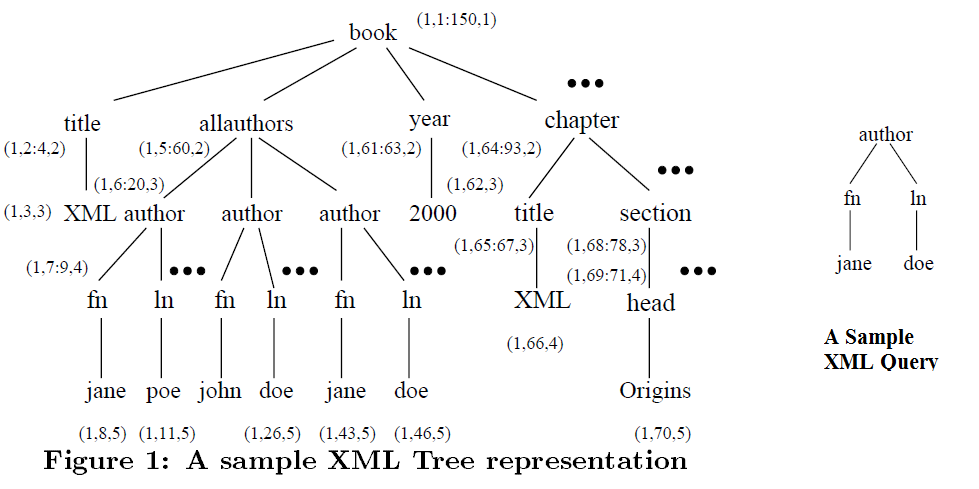
\includegraphics[width=\textwidth,height=0.65\textheight,keepaspectratio]{xmlalg-data.png} 
\footnote{\tiny{Изображение взято из \cite{Bruno2002}}}
\end{figure}    
\end{frame}

\begin{frame}
\frametitle{Наивный подход}

\begin{columns}
\begin{column}{0.25\textwidth}
{ \footnotesize
``В лоб'':
\begin{enumerate}
  \item Разбить запрос на бинарные отношения;
  \item Найти такие отношения в базе данных;
  \item Склеить результат.
\end{enumerate}

плохо, ибо промежуточных результатов может быть ОЧЕНЬ МНОГО, при том что входных и результирующих данных небольшое количество.
}
\end{column}
\begin{column}{0.75\textwidth}  %%<--- here

\begin{figure}[htb]
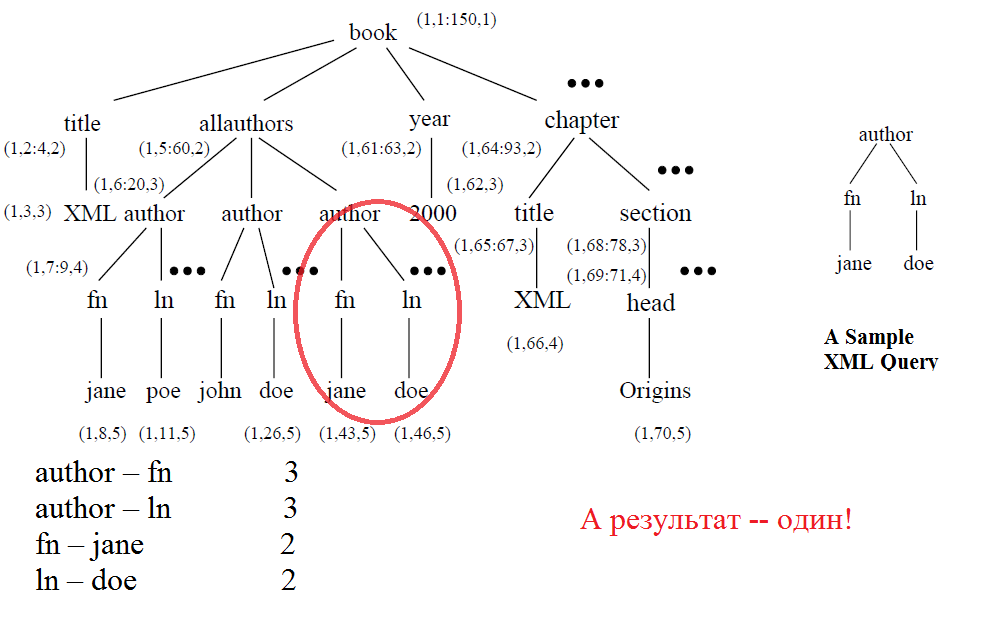
\includegraphics[width=\textwidth,height=0.65\textheight,keepaspectratio]{xmlalg-statistics.png} 
\footnote{\tiny{Изображение взято из \cite{Bruno2002}}}
\end{figure}    

\end{column}
\end{columns}
\end{frame}

\begin{frame}
\frametitle{Альтернатива: алгоритм PathStack}
Идея:
\begin{enumerate}
  %\setlength\itemsep{1em}
  \item Используем набор связанных друг с другом стеков;
  \item Каждый стек содержит частичные результаты;
  \item Полный результат получится ``правильным'' обходом стеков.
\end{enumerate}

\begin{figure}[htb]
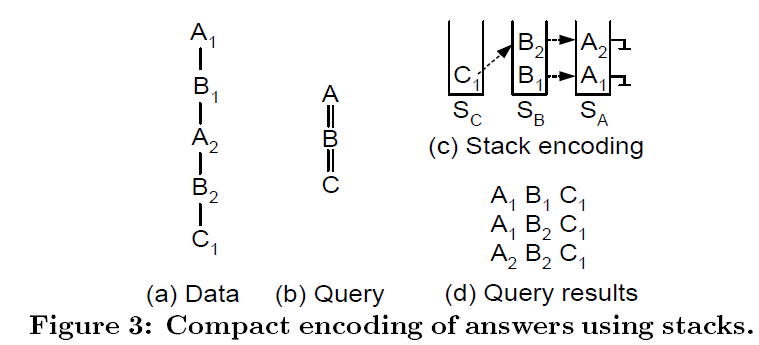
\includegraphics[width=\textwidth,height=0.50\textheight,keepaspectratio]{xmlalg-example.png} 
\footnote{\tiny{Изображение взято из \url{Bruno2002}}}
\end{figure}    

\end{frame}

\begin{noheadline}
\begin{frame}{Table of contents 2} 
\begin{figure}[htb]
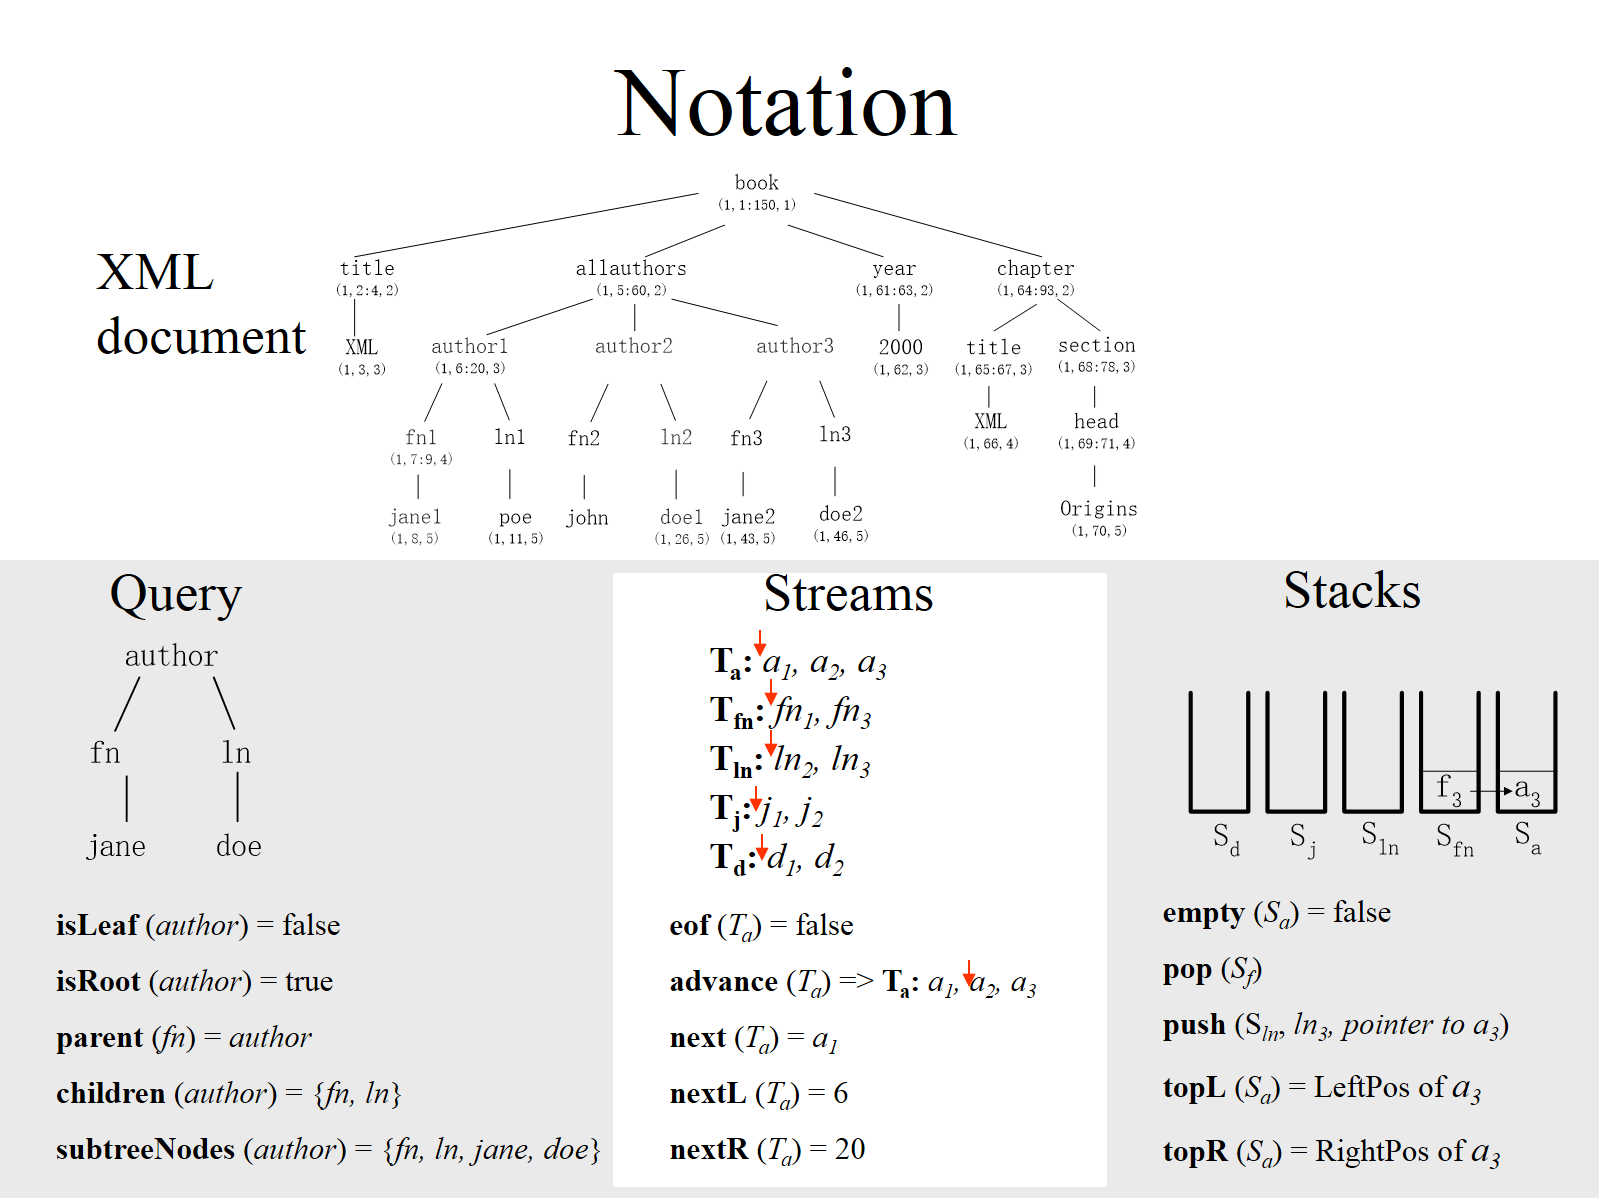
\includegraphics[width=\textwidth,height=0.85\textheight,keepaspectratio]{xmlalg-notation.png} 
\footnote{\tiny{Изображение взято из \url{http://www.cs.ucr.edu/~tsotras/cs236/W15/HolisticTwigJoin.ppt}}}
\end{figure}    

\end{frame}


\begin{frame}{Table of contents 2} 

\begin{columns}
\begin{column}{0.25\textwidth}

{ \footnotesize
Идея в общих чертах. В цикле, пока потоки не опустеют, брать узел с минимальным LeftPos и пушить в соответствующий стек. Как только получим лист~--- выдаем решения. 
}
\end{column}
\begin{column}{0.75\textwidth}  %%<--- here

\begin{figure}[htb]
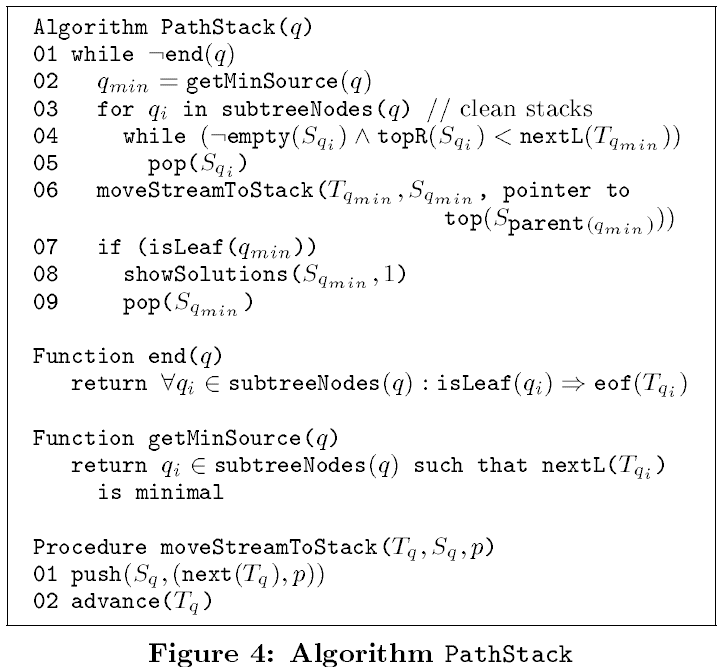
\includegraphics[width=\textwidth,height=0.85\textheight,keepaspectratio]{xmlalg-pathstack.png} 
\footnote{\tiny{Изображение взято из \cite{Bruno2002}}}
\end{figure}    

\end{column}
\end{columns}

\end{frame}

\begin{frame}{Table of contents 2} 
\begin{figure}[htb]
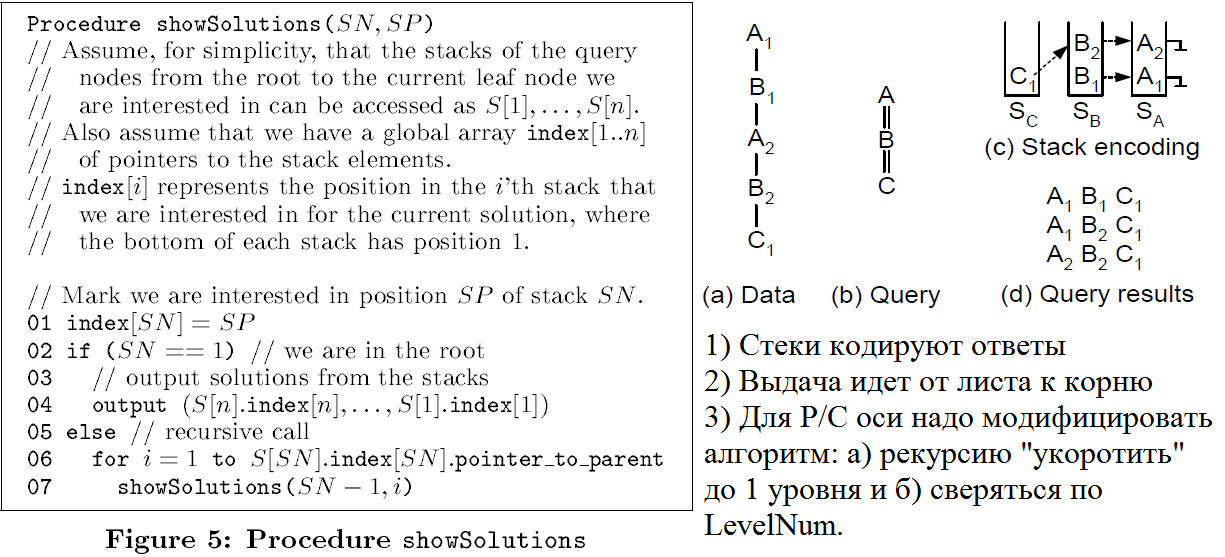
\includegraphics[width=\textwidth,height=0.85\textheight,keepaspectratio]{xmlalg-showsols.png} 
\footnote{\tiny{Изображение взято из \cite{Bruno2002}}}
\end{figure}    

\end{frame}

\end{noheadline}

\begin{frame}
\frametitle{Анализ алгоритма PathStack}

\begin{itemize}
  \setlength\itemsep{1em}
  \item Корректный: возвращает все значения, не возвращает ничего лишнего.
  \item В худшем случае PathStack имеет вычислительную сложность по I/O и CPU линейную от суммы размеров входных списков и выходного списка.
  \item \alert{Но! Лишние промежуточные результаты таки бывают :(}
\end{itemize}
\end{frame}

\begin{frame}
\frametitle{Пример:}

\begin{figure}[htb]
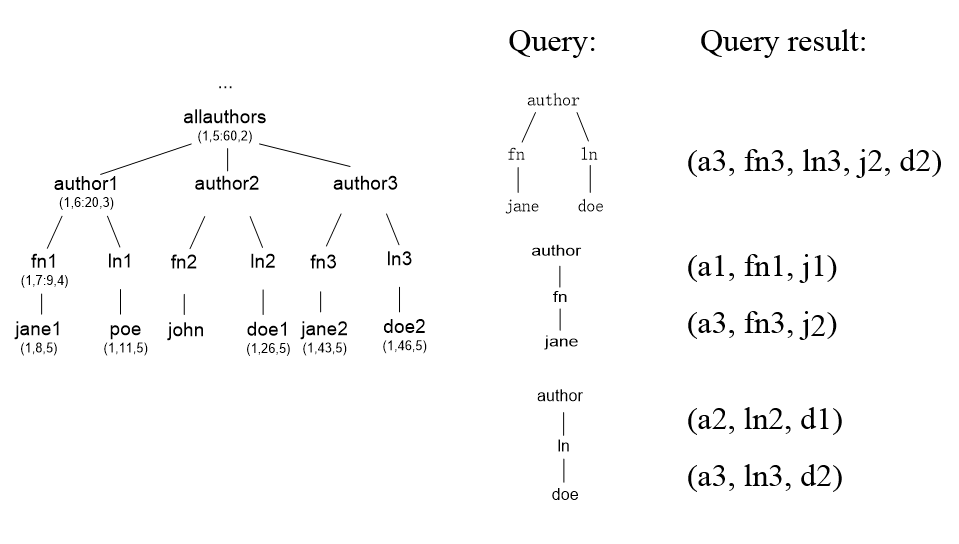
\includegraphics[width=\textwidth,height=0.85\textheight,keepaspectratio]{xmlalg-twigstack1.png} 
\footnote{\tiny{Изображение взято из \url{http://www.cs.ucr.edu/~tsotras/cs236/W15/HolisticTwigJoin.ppt}}}
\end{figure}    

\end{frame}

\begin{frame}
\frametitle{Идея TwigStack}

Идея: класть в стек только такие ноды, которые потом могут быть соединены с кем-то. 

\begin{itemize}
  \setlength\itemsep{1em}
  \item Перед тем как взять ноду $h_q$ из потока $T_q$ и положить в стек $S_q$ TwigStack используем getNext() чтобы проверить:
  \begin{enumerate}
    \setlength\itemsep{1em}
  
     \item что узел $h_q$ имеет потомка $h_{q_i}$ в каждом потоке $T_{q_i}$ для каждого $q_i \in children(q)$;
     \item каждая из нод $h_{q_i}$ рекурсивно удовлетворяет 1).
  \end{enumerate}

\end{itemize}
\end{frame}

\begin{frame}
\frametitle{Анализ алгоритма TwigStack}

\begin{itemize}
  \setlength\itemsep{1em}
  \item Корректный: возвращает все значения, не возвращает ничего лишнего.
  \item В худшем случае TwigStack имеет вычислительную сложность по I/O и CPU линейную от суммы размеров входных списков и выходного списка.
  \item В худшем сучае TwigStack имеет пространственную сложность вида минимум из 1) сумма размеров n входных списков и 2) n * максимальную длину пути от корня до листа в D.
  
\end{itemize}
\end{frame}

\begin{frame}
	\frametitle{Итог по XML}
	
	\begin{itemize}
		\setlength\itemsep{1em}
		\item Скорее мертв чем жив, отдельные СУБД на нем никого не интересуют, исследования завершены;
		\item Причины на 70\% связаны со сложностью XQuery, люди не стали его учить $\longrightarrow$ он не пошел в массы, нет пользователей;
		\item Оставшиеся 30\% это сложность вычисления запросов;
		\item Однако функционал включен во многие большие СУБД: есть и тип данных, и язык запросов поддерживается;
		\item Близится очередное пришествие языков для древовидных структур~--- для JSON, хотя там всё немного по-другому. Подробнее: JSONiq (кажется не взлетел), SQL++,  PartiQL, n1ql.
		
	\end{itemize}
\end{frame}

\begin{frame}[allowframebreaks]
\frametitle{Ссылки}
\footnotesize{
\begin{thebibliography}{99}

\bibitem[Jagadish et al., 2002] {Jagadish2002} H. V. Jagadish, S. Al-Khalifa, A. Chapman, L. V. S. Lakshmanan, A. Nierman, S. Paparizos, J. M. Patel, D. Srivastava, N. Wiwatwattana, Y. Wu, and C. Yu. 2002. TIMBER: A native XML database. The VLDB Journal 11, 4 (December 2002), 274--291. DOI=http://dx.doi.org/10.1007/s00778-002-0081-x 

\bibitem[Luna Dong and Divesh Srivastava, 2009] {Luna2009} Xin Luna Dong, Divesh Srivastava. XML Indexing. Encyclopedia of Database Systems. Springer US, 2009. 3585--3591. \url{http://dx.doi.org/10.1007/978-0-387-39940-9_779}

\bibitem[Grust et al., 2009] {Grust2009} Torsten Grust, H. V. Jagadish, Fatma Ozcan, Cong Yu. XQuery Processors. Encyclopedia of Database Systems. Springer US, 2009. 3671--3675.

\bibitem[Grust et al., 2004] {Grust2004} Torsten Grust, Sherif Sakr, and Jens Teubner. 2004. XQuery on SQL hosts. In Proceedings of the Thirtieth international conference on Very large data bases - Volume 30 (VLDB '04), Mario A. Nascimento, M. Tamer Özsu, Donald Kossmann, Renée J. Miller, José A. Blakeley, and K. Bernhard Schiefer (Eds.), Vol. 30. VLDB Endowment 252-263. 

\bibitem[Hidders and Paredaens, 2009] {Hidders2009} Jan Hidders and Jan Paredaens. XPath/XQuery. Encyclopedia of Database Systems. Springer US, 2009. 3659--3665.\url{http://dx.doi.org/10.1007/978-0-387-39940-9_774}

\bibitem[Taranov et al., 2010] {Taranov2010} Ilya Taranov, Ivan Shcheklein, Alexander Kalinin, Leonid Novak, Sergei Kuznetsov, Roman Pastukhov, Alexander Boldakov, Denis Turdakov, Konstantin Antipin, Andrey Fomichev, Peter Pleshachkov, Pavel Velikhov, Nikolai Zavaritski, Maxim Grinev, Maria Grineva, and Dmitry Lizorkin. 2010. Sedna: native XML database management system (internals overview). In Proceedings of the 2010 ACM SIGMOD International Conference on Management of data (SIGMOD '10). ACM, New York, NY, USA, 1037-1046. DOI=http://dx.doi.org/10.1145/1807167.1807282 

\bibitem[Bruno et al., 2002] {Bruno2002} Nicolas Bruno, Nick Koudas, and Divesh Srivastava. 2002. Holistic twig joins: optimal XML pattern matching. In Proceedings of the 2002 ACM SIGMOD international conference on Management of data (SIGMOD '02). ACM, New York, NY, USA, 310-321. DOI: https://doi.org/10.1145/564691.564727 

%\bibitem[Ivanova et al., 2010] {Ivanova2010} Milena G. Ivanova, Martin L. Kersten, Niels J. Nes, and Romulo A.P. Gonçalves. 2010. An architecture for recycling intermediates in a column-store. ACM Trans. Database Syst. 35, 4, Article 24 (October 2010), 43 pages. DOI=10.1145/1862919.1862921 http://doi.acm.org/10.1145/1862919.1862921 

%\bibitem[Shatdal et al., 1994] {Shatdal1994} Ambuj Shatdal, Chander Kant, and Jeffrey F. Naughton. 1994. Cache Conscious Algorithms for Relational Query Processing. In Proceedings of the 20th International Conference on Very Large Data Bases (VLDB '94), Jorge B. Bocca, Matthias Jarke, and Carlo Zaniolo (Eds.). Morgan Kaufmann Publishers Inc., San Francisco, CA, USA, 510--521. 

%\bibitem[Boncz et al., 2008] {Boncz2008} Peter A. Boncz, Martin L. Kersten, and Stefan Manegold. 2008. Breaking the memory wall in MonetDB. Commun. ACM 51, 12 (December 2008), 77--85. DOI=http://dx.doi.org/10.1145/1409360.1409380 

%\bibitem[Boncz et al., 2005] {Boncz2005} Peter Boncz, Marcin Zukowski, Niels Nes. MonetDB/X100: Hyper-Pipelining Query Execution. CIDR'05.

%\bibitem[Hennessy and Patterson, 2011] {Hennessy2011}  John L. Hennessy and David A. Patterson. 2011. Computer Architecture, Fifth Edition: A Quantitative Approach (5th ed.). Morgan Kaufmann Publishers Inc., San Francisco, CA, USA. 

%\bibitem[Tsirogiannis et al., 2009] {Tsirogiannis2009}  Dimitris Tsirogiannis, Stavros Harizopoulos, Mehul A. Shah, Janet L. Wiener, and Goetz Graefe. 2009. Query processing techniques for solid state drives. In Proceedings of the 2009 ACM SIGMOD International Conference on Management of data (SIGMOD '09), Carsten Binnig and Benoit Dageville (Eds.). ACM, New York, NY, USA, 59-72. DOI=http://dx.doi.org/10.1145/1559845.1559854 

%\bibitem[Li and Ross, 1999] {Li1999} Zhe Li and Kenneth A. Ross. 1999. Fast joins using join indices. The VLDB Journal 8, 1 (April 1999), 1--24. DOI=http://dx.doi.org/10.1007/s007780050071 

%\bibitem[Star Schema Benchmark Specification, 2009] {SSB} Star Schema Benchmark. Revision 3, June 5, 2009 Pat O'Neil, Betty O'Neil, Xuedong Chen

%\bibitem[Abadi et al., 2008] {Abadi2008} Daniel J. Abadi, Samuel R. Madden, and Nabil Hachem. 2008. Column-stores vs. row-stores: how different are they really?. In Proceedings of the 2008 ACM SIGMOD international conference on Management of data (SIGMOD '08). ACM, New York, NY, USA, 967-980. DOI=http://dx.doi.org/10.1145/1376616.1376712 

%\bibitem[TPC-H Specification, 2011] {TPC-H} TPC BENCHMARK(TM) H (Decision Support) Standard Specification Revision 2.14.2

%\bibitem[Abadi et al., 2012] {Abadi2013} Daniel Abadi, Peter Boncz, Stavros Harizopoulos. The Design and Implementation of Modern Column-Oriented Database Systems. Foundations and Trends(R) in Databases Vol. 5, No. 3 (2012) 197--280

%\bibitem[Harizopoulos et al., 2009] {Harizopoulos2009} Stavros Harizopoulos, Daniel Abadi, Peter Boncz. Column-Oriented Database Systems. VLDB 2009 Tutorial (slides).

% \bibitem[Чернышев, 2013] {Chernishev2013}	Г. А. Чернышев, <<Организация физического уровня колоночных СУБД>>, Тр. СПИИРАН, 30 (2013), 204--222

% \bibitem[Кузнецов, 2010] {Kuznetsov2010}	 Кузнецов С.Д., <<Год эпохи перемен в технологии баз данных>>, Труды Института системного программирования РАН, 19 (2010), 9--34

%\bibitem[Elnikety, 2009] {Elnikety2009} Distributed DBMS. Sameh Elnikety. Encyclopedia of Database Systems. Ling Liu and M. Tamer {\"O}zsu (eds), p. 896--899. Springer US, 2009. \url{http://dx.doi.org/10.1007/978-0-387-39940-9\_654}

%\bibitem[Kian-Lee Tan, 2009] {Kian-Lee2009} Distributed Database Systems. Kian-Lee Tan. Encyclopedia of Database Systems. Ling Liu and M. Tamer {\"O}zsu (eds), p. 894--896. Springer US, 2009. \url{http://dx.doi.org/10.1007/978-0-387-39940-9_701}

%\bibitem[{\"O}zsu and Valduriez, 2009] {Ozsu2011} {\"O}zsu M.T. and Valduriez P. Principles of Distributed Database Systems, 3rd ed. Prentice-Hall, 2011.

%\bibitem[Kossmann, 2000] {Kossmann2000} Donald Kossmann. 2000. The state of the art in distributed query processing. ACM Comput. Surv. 32, 4 (December 2000), 422--469. DOI=http://dx.doi.org/10.1145/371578.371598 


%\bibitem[Ioannidis, 2003] {Ioannidis2003}  Yannis Ioannidis. 2003. The history of histograms (abridged). In Proceedings of the 29th international conference on Very large data bases - Volume 29 (VLDB '03), Johann Christoph Freytag, Peter C. Lockemann, Serge Abiteboul, Michael J. Carey, Patricia G. Selinger, and Andreas Heuer (Eds.), Vol. 29. VLDB Endowment 19--30. 

%\bibitem[Ioannidis and Poosala, 1995] {Ioannidis1995} Y. Ioannidis and V. Poosala. Histogram Based Solutions to Diverse Database Estimation Problems, IEEE Data Engineering, Vol. 18, No. 3, pp. 10--18, September 1995.

%\bibitem[Poosala et al., 1996] {Poosala1996} Viswanath Poosala, Peter J. Haas, Yannis E. Ioannidis, and Eugene J. Shekita. 1996. Improved histograms for selectivity estimation of range predicates. In Proceedings of the 1996 ACM SIGMOD international conference on Management of data (SIGMOD '96), Jennifer Widom (Ed.). ACM, New York, NY, USA, 294--305. DOI=http://dx.doi.org/10.1145/233269.233342 


%\bibitem[Kooi, 1980] {Kooi1980} Robert Philip Kooi. The Optimization of Queries in Relational Databases. PhD Thesis, Case Western Reserve University (1980).

%\bibitem[Piatetsky-Shapiro and Connel, 1984] {Piatetsky-Shapiro1984} Gregory Piatetsky-Shapiro and Charles Connell. 1984. Accurate estimation of the number of tuples satisfying a condition. In Proceedings of the 1984 ACM SIGMOD international conference on Management of data (SIGMOD '84). ACM, New York, NY, USA, 256--276. DOI=http://dx.doi.org/10.1145/602259.602294 


%\bibitem[Garcia-Molina et al., 2004] {Ulman2004} Гектор Гарсиа-Молина, Джеффри Д. Ульман, Дженнифер Уидом. Системы баз данных. Полный курс.  ISBN 5-8459-0384-Х; 2004 г. 

%\bibitem[Hellerstein et al., 2007] {Hellerstein2007} Joseph M. Hellerstein, Michael Stonebraker, and James Hamilton. Architecture of a Database System. Found. Trends databases 1, 2 (February 2007), 141--259. 

%\bibitem[Neumann, 2009] {Neumann2009} Thomas Neumann. Query Optimization (in Relational Databases). Encyclopedia of Database Systems. Springer US, 2009. 2273--2278.\url{http://dx.doi.org/10.1007/978-0-387-39940-9_293}

%\bibitem[Selinger et al., 1979] {Selinger1979} Selinger P.G., Astrahan M.M., Chamberlin D.D., Lorie R.A., and Price T.G. Access path selection in a relational database management System. In Proc. ACM SIGMOD Int. Conf. on Management of Data, 1979, pp. 23--34.

%\bibitem[Haas et al., 1989] {Haas1989} Haas L.M., Freytag J.C., Lohman G.M., and Pirahesh H. Extensible query processing in starburst. In Proc. ACM SIGMOD Int. Conf. on Management of Data, 1989, pp. 377--388.

%\bibitem[Graefe, 1995] {Graefe1995} Graefe G. The cascades framework for query optimization. Q. Bull. IEEE TC on Data Engineering, 18(3):19--29, 1995.

%\bibitem[Graefe and McKenna, 1993] {Graefe1993} Graefe G. and McKenna W.J. The volcano optimizer generator: Extensibility and efficient search. In Proc. 9th Int. Conf. on Data Engineering, 1993, pp. 209--218.

%\bibitem[Chaudhuri, 1998] {Chaudhuri1998} Chaudhuri S. An overview of query optimization in relational systems. In Proc. 17th ACM SIGACT-SIGMOD-SIGART Symp. Principles of Database Systems, 1998, pp. 34--43.

%\bibitem[Ioannidis, 1996] {Ioannidis1996} Ioannidis Y. Query optimization. In Handbook of Computer Science, A.B. Tucker (ed.). CRC Press, 1996.

%\bibitem[Jarke and Koch, 1984] {Chaudhuri1984} Jarke M. and Koch J. Query optimization in database systems. ACM Comput. Surv., 16(2):111–152, 1984.

%\bibitem[Ioannidis, 1996] {Ioannidis1996} Yannis E. Ioannidis. 1996. Query optimization. ACM Comput. Surv. 28, 1 (March 1996), 121--123. DOI=http://dx.doi.org/10.1145/234313.234367 

%\bibitem[Graefe, 1996] {Graefe1996} Goetz Graefe. 1996. Iterators, schedulers, and distributed-memory parallelism. Softw. Pract. Exper. 26, 4 (April 1996), 427--452. DOI=http://dx.doi.org/10.1002/(SICI)1097-024X(199604)26:4<427::AID-SPE20>3.3.CO;2-8 

%\bibitem[Taniar et al., 2008] {Taniar2008} David Taniar, Clement H. C. Leung, Wenny Rahayu, and Sushant Goel. 2008. High Performance Parallel Database Processing and Grid Databases. Wiley Publishing. 

%\bibitem[Ramakrishnan and Gehrke, 2000] {Ramakrishnan2000}  Raghu Ramakrishnan and Johannes Gehrke. 2000. Database Management Systems (2nd ed.). Osborne/McGraw-Hill, Berkeley, CA, USA. 

\end{thebibliography}
}
\end{frame}


\end{document} 